\documentclass[11pt,a4paper]{article}

\usepackage[a4paper,left=3.5cm, right=2.5cm, top=3.5cm, bottom=3.5cm]{geometry}
\usepackage[dutch]{babel}
\usepackage{amsmath}
\usepackage{tikz}
\usepackage{graphicx}

\setlength\parindent{0pt}                   % Fix stupid indentation on new line
\setlength\parskip{\medskipamount}

\title{Inloopverslag Masterproef}
\author{Olivier Van den Eede}
\date{}

\begin{document}
    \maketitle
    
    \section{Voorlopige titel}
        De Gekozen titel zal gehouden worden op `Visie voor semantische robotnavigatie in ziekhuisgangen`.

    \section{Contactgegevens}
        \begin{table}[h]
            \begin{tabular}{l | l}
                Student: & Bedrijf: \\ \hline
                Olivier Van den Eede & Filip Reniers \\
                Edegemsesteenweg 151 & Celestijnenlaan 300 - bus 2420 \\
                2550 Kontich & 3001 Leuven \\
                olivier.vandeneede@student.kuleuven.be & filip.reniers@kuleuven.be \\
                0476/20.78.49 & \\
            \end{tabular}
        \end{table}

    \section{Doelstellingen}

    % Het doel van deze thesis is om een set van feature detectors te selecteren en configureren om de samenstellende componenten/onderdelen van objecten te herkennen. 
    % Meerbepaald de objecten die terug te vinden zijn in de gangen van de logistieke vloer van een ziekenhuis.

    Het doel van deze masterproef is te onderzoeken welke objecten/features er aanwezig zijn in de logistieke gangen van een ziekenhuis die bruikbaar kunnen zijn om een route door de gangen te beschrijven door middel van een semantische kaart.
    
    Er zal onderzocht worden wat de beste techniek is om deze objecten/features te detecteren en te tracken vanop een bewegende robot. Het resultaat zal weergegeven worden op de kaart en het genomen beeld.
    
    In tweede instantie zal er getracht worden om op basis van de semantise kaart en de gedetecteerde objecten in een beeld, de actuele locatie van de robot te volgen.
    De robot begint hierbij steeds op een gekende locatie, dus gaat het over navigatie doorheen de gangen.

    \section{Reeds uitgevoerde activiteiten}
        \begin{itemize}
            \item Opzoeken van relevante literatuur~\cite{844076}~\cite{Yi2009ActivesemanticLW}~\cite{7780460}~\cite{Se02mobilerobot}~\cite{semloc}
        \end{itemize}


    \begin{figure}[htbp]
        \centering
        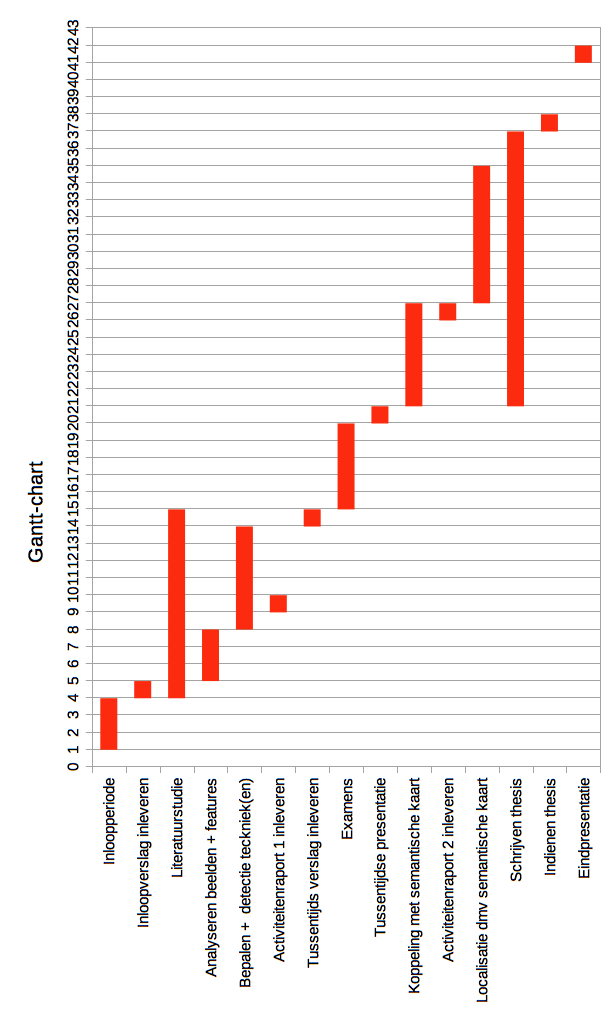
\includegraphics[]{planning.png}
        \caption{Planning}
    \end{figure}

    \bibliographystyle{plain}
    \bibliography{bibtex.bib}

\end{document}